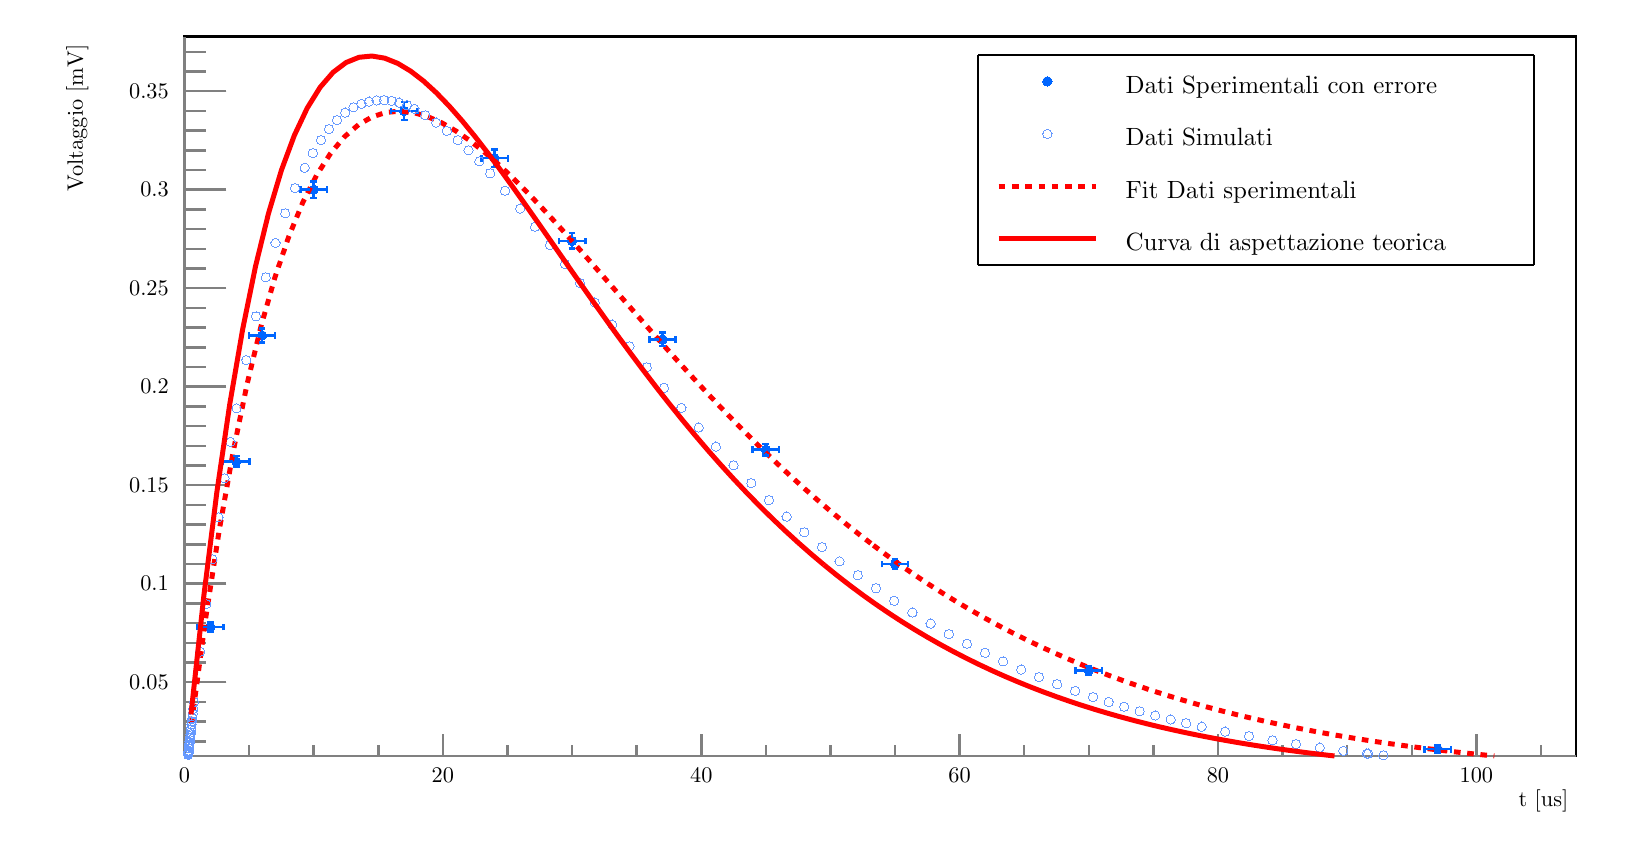
\begin{tikzpicture}
\pgfdeclareplotmark{cross} {
\pgfpathmoveto{\pgfpoint{-0.3\pgfplotmarksize}{\pgfplotmarksize}}
\pgfpathlineto{\pgfpoint{+0.3\pgfplotmarksize}{\pgfplotmarksize}}
\pgfpathlineto{\pgfpoint{+0.3\pgfplotmarksize}{0.3\pgfplotmarksize}}
\pgfpathlineto{\pgfpoint{+1\pgfplotmarksize}{0.3\pgfplotmarksize}}
\pgfpathlineto{\pgfpoint{+1\pgfplotmarksize}{-0.3\pgfplotmarksize}}
\pgfpathlineto{\pgfpoint{+0.3\pgfplotmarksize}{-0.3\pgfplotmarksize}}
\pgfpathlineto{\pgfpoint{+0.3\pgfplotmarksize}{-1.\pgfplotmarksize}}
\pgfpathlineto{\pgfpoint{-0.3\pgfplotmarksize}{-1.\pgfplotmarksize}}
\pgfpathlineto{\pgfpoint{-0.3\pgfplotmarksize}{-0.3\pgfplotmarksize}}
\pgfpathlineto{\pgfpoint{-1.\pgfplotmarksize}{-0.3\pgfplotmarksize}}
\pgfpathlineto{\pgfpoint{-1.\pgfplotmarksize}{0.3\pgfplotmarksize}}
\pgfpathlineto{\pgfpoint{-0.3\pgfplotmarksize}{0.3\pgfplotmarksize}}
\pgfpathclose
\pgfusepathqstroke
}
\pgfdeclareplotmark{cross*} {
\pgfpathmoveto{\pgfpoint{-0.3\pgfplotmarksize}{\pgfplotmarksize}}
\pgfpathlineto{\pgfpoint{+0.3\pgfplotmarksize}{\pgfplotmarksize}}
\pgfpathlineto{\pgfpoint{+0.3\pgfplotmarksize}{0.3\pgfplotmarksize}}
\pgfpathlineto{\pgfpoint{+1\pgfplotmarksize}{0.3\pgfplotmarksize}}
\pgfpathlineto{\pgfpoint{+1\pgfplotmarksize}{-0.3\pgfplotmarksize}}
\pgfpathlineto{\pgfpoint{+0.3\pgfplotmarksize}{-0.3\pgfplotmarksize}}
\pgfpathlineto{\pgfpoint{+0.3\pgfplotmarksize}{-1.\pgfplotmarksize}}
\pgfpathlineto{\pgfpoint{-0.3\pgfplotmarksize}{-1.\pgfplotmarksize}}
\pgfpathlineto{\pgfpoint{-0.3\pgfplotmarksize}{-0.3\pgfplotmarksize}}
\pgfpathlineto{\pgfpoint{-1.\pgfplotmarksize}{-0.3\pgfplotmarksize}}
\pgfpathlineto{\pgfpoint{-1.\pgfplotmarksize}{0.3\pgfplotmarksize}}
\pgfpathlineto{\pgfpoint{-0.3\pgfplotmarksize}{0.3\pgfplotmarksize}}
\pgfpathclose
\pgfusepathqfillstroke
}
\pgfdeclareplotmark{newstar} {
\pgfpathmoveto{\pgfqpoint{0pt}{\pgfplotmarksize}}
\pgfpathlineto{\pgfqpointpolar{44}{0.5\pgfplotmarksize}}
\pgfpathlineto{\pgfqpointpolar{18}{\pgfplotmarksize}}
\pgfpathlineto{\pgfqpointpolar{-20}{0.5\pgfplotmarksize}}
\pgfpathlineto{\pgfqpointpolar{-54}{\pgfplotmarksize}}
\pgfpathlineto{\pgfqpointpolar{-90}{0.5\pgfplotmarksize}}
\pgfpathlineto{\pgfqpointpolar{234}{\pgfplotmarksize}}
\pgfpathlineto{\pgfqpointpolar{198}{0.5\pgfplotmarksize}}
\pgfpathlineto{\pgfqpointpolar{162}{\pgfplotmarksize}}
\pgfpathlineto{\pgfqpointpolar{134}{0.5\pgfplotmarksize}}
\pgfpathclose
\pgfusepathqstroke
}
\pgfdeclareplotmark{newstar*} {
\pgfpathmoveto{\pgfqpoint{0pt}{\pgfplotmarksize}}
\pgfpathlineto{\pgfqpointpolar{44}{0.5\pgfplotmarksize}}
\pgfpathlineto{\pgfqpointpolar{18}{\pgfplotmarksize}}
\pgfpathlineto{\pgfqpointpolar{-20}{0.5\pgfplotmarksize}}
\pgfpathlineto{\pgfqpointpolar{-54}{\pgfplotmarksize}}
\pgfpathlineto{\pgfqpointpolar{-90}{0.5\pgfplotmarksize}}
\pgfpathlineto{\pgfqpointpolar{234}{\pgfplotmarksize}}
\pgfpathlineto{\pgfqpointpolar{198}{0.5\pgfplotmarksize}}
\pgfpathlineto{\pgfqpointpolar{162}{\pgfplotmarksize}}
\pgfpathlineto{\pgfqpointpolar{134}{0.5\pgfplotmarksize}}
\pgfpathclose
\pgfusepathqfillstroke
}
\definecolor{c}{rgb}{1,1,1};
\draw [color=c, fill=c] (0,0) rectangle (20,10.2882);
\draw [color=c, fill=c] (1.98506,1.04589) rectangle (19.6585,10.1814);
\definecolor{c}{rgb}{0,0,0};
\draw [c,line width=0.9] (1.98506,1.04589) -- (1.98506,10.1814) -- (19.6585,10.1814) -- (19.6585,1.04589) -- (1.98506,1.04589);
\definecolor{c}{rgb}{1,1,1};
\draw [color=c, fill=c] (1.98506,1.04589) rectangle (19.6585,10.1814);
\definecolor{c}{rgb}{0,0,0};
\draw [c,line width=0.9] (1.98506,1.04589) -- (1.98506,10.1814) -- (19.6585,10.1814) -- (19.6585,1.04589) -- (1.98506,1.04589);
\definecolor{c}{rgb}{0.5,0.5,0.5};
\draw [c,line width=0.9] (1.98506,1.04589) -- (19.6585,1.04589);
\draw [c,line width=0.9] (1.98506,1.31863) -- (1.98506,1.04589);
\draw [c,line width=0.9] (2.80536,1.18226) -- (2.80536,1.04589);
\draw [c,line width=0.9] (3.62567,1.18226) -- (3.62567,1.04589);
\draw [c,line width=0.9] (4.44597,1.18226) -- (4.44597,1.04589);
\draw [c,line width=0.9] (5.26628,1.31863) -- (5.26628,1.04589);
\draw [c,line width=0.9] (6.08658,1.18226) -- (6.08658,1.04589);
\draw [c,line width=0.9] (6.90689,1.18226) -- (6.90689,1.04589);
\draw [c,line width=0.9] (7.72719,1.18226) -- (7.72719,1.04589);
\draw [c,line width=0.9] (8.5475,1.31863) -- (8.5475,1.04589);
\draw [c,line width=0.9] (9.3678,1.18226) -- (9.3678,1.04589);
\draw [c,line width=0.9] (10.1881,1.18226) -- (10.1881,1.04589);
\draw [c,line width=0.9] (11.0084,1.18226) -- (11.0084,1.04589);
\draw [c,line width=0.9] (11.8287,1.31863) -- (11.8287,1.04589);
\draw [c,line width=0.9] (12.649,1.18226) -- (12.649,1.04589);
\draw [c,line width=0.9] (13.4693,1.18226) -- (13.4693,1.04589);
\draw [c,line width=0.9] (14.2896,1.18226) -- (14.2896,1.04589);
\draw [c,line width=0.9] (15.1099,1.31863) -- (15.1099,1.04589);
\draw [c,line width=0.9] (15.9302,1.18226) -- (15.9302,1.04589);
\draw [c,line width=0.9] (16.7505,1.18226) -- (16.7505,1.04589);
\draw [c,line width=0.9] (17.5709,1.18226) -- (17.5709,1.04589);
\draw [c,line width=0.9] (18.3912,1.31863) -- (18.3912,1.04589);
\draw [c,line width=0.9] (18.3912,1.31863) -- (18.3912,1.04589);
\draw [c,line width=0.9] (19.2115,1.18226) -- (19.2115,1.04589);
\definecolor{c}{rgb}{0,0,0};
\draw [anchor=base] (1.98506,0.706382) node[scale=0.805902, color=c, rotate=0]{0};
\draw [anchor=base] (5.26628,0.706382) node[scale=0.805902, color=c, rotate=0]{20};
\draw [anchor=base] (8.5475,0.706382) node[scale=0.805902, color=c, rotate=0]{40};
\draw [anchor=base] (11.8287,0.706382) node[scale=0.805902, color=c, rotate=0]{60};
\draw [anchor=base] (15.1099,0.706382) node[scale=0.805902, color=c, rotate=0]{80};
\draw [anchor=base] (18.3912,0.706382) node[scale=0.805902, color=c, rotate=0]{100};
\draw [anchor= east] (19.6585,0.469755) node[scale=0.805902, color=c, rotate=0]{t [us]};
\definecolor{c}{rgb}{0.5,0.5,0.5};
\draw [c,line width=0.9] (1.98506,1.04589) -- (1.98506,10.1814);
\draw [c,line width=0.9] (2.51784,1.98272) -- (1.98506,1.98272);
\draw [c,line width=0.9] (2.25145,2.23291) -- (1.98506,2.23291);
\draw [c,line width=0.9] (2.25145,2.48309) -- (1.98506,2.48309);
\draw [c,line width=0.9] (2.25145,2.73328) -- (1.98506,2.73328);
\draw [c,line width=0.9] (2.25145,2.98346) -- (1.98506,2.98346);
\draw [c,line width=0.9] (2.51784,3.23364) -- (1.98506,3.23364);
\draw [c,line width=0.9] (2.25145,3.48383) -- (1.98506,3.48383);
\draw [c,line width=0.9] (2.25145,3.73401) -- (1.98506,3.73401);
\draw [c,line width=0.9] (2.25145,3.9842) -- (1.98506,3.9842);
\draw [c,line width=0.9] (2.25145,4.23438) -- (1.98506,4.23438);
\draw [c,line width=0.9] (2.51784,4.48457) -- (1.98506,4.48457);
\draw [c,line width=0.9] (2.25145,4.73475) -- (1.98506,4.73475);
\draw [c,line width=0.9] (2.25145,4.98494) -- (1.98506,4.98494);
\draw [c,line width=0.9] (2.25145,5.23512) -- (1.98506,5.23512);
\draw [c,line width=0.9] (2.25145,5.48531) -- (1.98506,5.48531);
\draw [c,line width=0.9] (2.51784,5.73549) -- (1.98506,5.73549);
\draw [c,line width=0.9] (2.25145,5.98568) -- (1.98506,5.98568);
\draw [c,line width=0.9] (2.25145,6.23586) -- (1.98506,6.23586);
\draw [c,line width=0.9] (2.25145,6.48604) -- (1.98506,6.48604);
\draw [c,line width=0.9] (2.25145,6.73623) -- (1.98506,6.73623);
\draw [c,line width=0.9] (2.51784,6.98641) -- (1.98506,6.98641);
\draw [c,line width=0.9] (2.25145,7.2366) -- (1.98506,7.2366);
\draw [c,line width=0.9] (2.25145,7.48678) -- (1.98506,7.48678);
\draw [c,line width=0.9] (2.25145,7.73697) -- (1.98506,7.73697);
\draw [c,line width=0.9] (2.25145,7.98715) -- (1.98506,7.98715);
\draw [c,line width=0.9] (2.51784,8.23734) -- (1.98506,8.23734);
\draw [c,line width=0.9] (2.25145,8.48752) -- (1.98506,8.48752);
\draw [c,line width=0.9] (2.25145,8.73771) -- (1.98506,8.73771);
\draw [c,line width=0.9] (2.25145,8.98789) -- (1.98506,8.98789);
\draw [c,line width=0.9] (2.25145,9.23808) -- (1.98506,9.23808);
\draw [c,line width=0.9] (2.51784,9.48826) -- (1.98506,9.48826);
\draw [c,line width=0.9] (2.51784,1.98272) -- (1.98506,1.98272);
\draw [c,line width=0.9] (2.25145,1.73254) -- (1.98506,1.73254);
\draw [c,line width=0.9] (2.25145,1.48235) -- (1.98506,1.48235);
\draw [c,line width=0.9] (2.25145,1.23217) -- (1.98506,1.23217);
\draw [c,line width=0.9] (2.51784,9.48826) -- (1.98506,9.48826);
\draw [c,line width=0.9] (2.25145,9.73844) -- (1.98506,9.73844);
\draw [c,line width=0.9] (2.25145,9.98863) -- (1.98506,9.98863);
\definecolor{c}{rgb}{0,0,0};
\draw [anchor= east] (1.88506,1.98272) node[scale=0.805902, color=c, rotate=0]{0.05};
\draw [anchor= east] (1.88506,3.23364) node[scale=0.805902, color=c, rotate=0]{0.1};
\draw [anchor= east] (1.88506,4.48457) node[scale=0.805902, color=c, rotate=0]{0.15};
\draw [anchor= east] (1.88506,5.73549) node[scale=0.805902, color=c, rotate=0]{0.2};
\draw [anchor= east] (1.88506,6.98641) node[scale=0.805902, color=c, rotate=0]{0.25};
\draw [anchor= east] (1.88506,8.23734) node[scale=0.805902, color=c, rotate=0]{0.3};
\draw [anchor= east] (1.88506,9.48826) node[scale=0.805902, color=c, rotate=0]{0.35};
\draw [anchor= east] (0.623372,10.1814) node[scale=0.805902, color=c, rotate=90]{Voltaggio [mV]};
\definecolor{c}{rgb}{0,0.4,1};
\foreach \P in {(2.31318,2.68324), (2.6413,4.78479), (2.96942,6.38597), (3.62567,8.23734), (4.7741,9.23808), (5.92252,8.63763), (6.90689,7.58686), (8.05531,6.33593), (9.3678,4.9349), (11.0084,3.48383), (13.4693,2.13283), (17.899,1.13209)}{\draw[mark
 options={color=c,fill=c},mark size=1.681682pt, line width=0.000000pt, mark=*] plot coordinates {\P};}
\definecolor{c}{rgb}{1,0,0};
\draw [c,dash pattern=on 2.40pt off 2.40pt ,line width=1.8] (2.07343,1.4579) -- (2.25016,2.77322) -- (2.42689,3.92037) -- (2.60363,4.91529) -- (2.78036,5.77257) -- (2.9571,6.5056) -- (3.13383,7.12659) -- (3.31057,7.64674) -- (3.4873,8.07627) --
 (3.66403,8.42451) -- (3.84077,8.69999) -- (4.0175,8.91046) -- (4.19424,9.06302) -- (4.37097,9.16411) -- (4.54771,9.2196) -- (4.72444,9.23482) -- (4.90117,9.21461) -- (5.07791,9.16336) -- (5.25464,9.08506) -- (5.43138,8.9833) -- (5.60811,8.86135) --
 (5.78485,8.72214) -- (5.96158,8.56833) -- (6.13831,8.4023) -- (6.31505,8.22618) -- (6.49178,8.04191) -- (6.66852,7.85121) -- (6.84525,7.65561) -- (7.02199,7.45648) -- (7.19872,7.25504) -- (7.37545,7.05235) -- (7.55219,6.84939) -- (7.72892,6.64697)
 -- (7.90566,6.44583) -- (8.08239,6.24662) -- (8.25912,6.04988) -- (8.43586,5.85609) -- (8.61259,5.66565) -- (8.78933,5.47892) -- (8.96606,5.29617) -- (9.1428,5.11764) -- (9.31953,4.94353) -- (9.49626,4.77398) -- (9.673,4.6091) -- (9.84973,4.44899)
 -- (10.0265,4.29369) -- (10.2032,4.14323) -- (10.3799,3.99761) -- (10.5567,3.85683) -- (10.7334,3.72084);
\draw [c,dash pattern=on 2.40pt off 2.40pt ,line width=1.8] (10.7334,3.72084) -- (10.9101,3.5896) -- (11.0869,3.46305) -- (11.2636,3.34112) -- (11.4403,3.22374) -- (11.6171,3.1108) -- (11.7938,3.00221) -- (11.9705,2.89788) -- (12.1473,2.79769) --
 (12.324,2.70155) -- (12.5007,2.60932) -- (12.6775,2.52091) -- (12.8542,2.4362) -- (13.0309,2.35507) -- (13.2077,2.27741) -- (13.3844,2.20309) -- (13.5612,2.13202) -- (13.7379,2.06406) -- (13.9146,1.99912) -- (14.0914,1.93708) -- (14.2681,1.87783) --
 (14.4448,1.82127) -- (14.6216,1.76729) -- (14.7983,1.71579) -- (14.975,1.66668) -- (15.1518,1.61985) -- (15.3285,1.57522) -- (15.5052,1.53269) -- (15.682,1.49217) -- (15.8587,1.45359) -- (16.0354,1.41685) -- (16.2122,1.38187) -- (16.3889,1.34859) --
 (16.5656,1.31693) -- (16.7424,1.2868) -- (16.9191,1.25816) -- (17.0958,1.23092) -- (17.2726,1.20503) -- (17.4493,1.18042) -- (17.626,1.15703) -- (17.8028,1.13481) -- (17.9795,1.11371) -- (18.1562,1.09366) -- (18.333,1.07463) -- (18.5097,1.05656) --
 (18.6196,1.04589);
\definecolor{c}{rgb}{0,0.4,1};
\draw [c,line width=0.9] (2.27049,2.68324) -- (2.14574,2.68324);
\draw [c,line width=0.9] (2.14574,2.64055) -- (2.14574,2.72593);
\draw [c,line width=0.9] (2.35587,2.68324) -- (2.48062,2.68324);
\draw [c,line width=0.9] (2.48062,2.64055) -- (2.48062,2.72593);
\draw [c,line width=0.9] (2.31318,2.72593) -- (2.31318,2.73962);
\draw [c,line width=0.9] (2.27049,2.73962) -- (2.35587,2.73962);
\draw [c,line width=0.9] (2.31318,2.64055) -- (2.31318,2.62685);
\draw [c,line width=0.9] (2.27049,2.62685) -- (2.35587,2.62685);
\draw [c,line width=0.9] (2.59861,4.78479) -- (2.47386,4.78479);
\draw [c,line width=0.9] (2.47386,4.7421) -- (2.47386,4.82748);
\draw [c,line width=0.9] (2.68399,4.78479) -- (2.80875,4.78479);
\draw [c,line width=0.9] (2.80875,4.7421) -- (2.80875,4.82748);
\draw [c,line width=0.9] (2.6413,4.82748) -- (2.6413,4.85601);
\draw [c,line width=0.9] (2.59861,4.85601) -- (2.68399,4.85601);
\draw [c,line width=0.9] (2.6413,4.7421) -- (2.6413,4.71357);
\draw [c,line width=0.9] (2.59861,4.71357) -- (2.68399,4.71357);
\draw [c,line width=0.9] (2.92673,6.38597) -- (2.80198,6.38597);
\draw [c,line width=0.9] (2.80198,6.34328) -- (2.80198,6.42866);
\draw [c,line width=0.9] (3.01211,6.38597) -- (3.13687,6.38597);
\draw [c,line width=0.9] (3.13687,6.34328) -- (3.13687,6.42866);
\draw [c,line width=0.9] (2.96942,6.42866) -- (2.96942,6.47201);
\draw [c,line width=0.9] (2.92673,6.47201) -- (3.01211,6.47201);
\draw [c,line width=0.9] (2.96942,6.34328) -- (2.96942,6.29993);
\draw [c,line width=0.9] (2.92673,6.29993) -- (3.01211,6.29993);
\draw [c,line width=0.9] (3.58298,8.23734) -- (3.45822,8.23734);
\draw [c,line width=0.9] (3.45822,8.19465) -- (3.45822,8.28003);
\draw [c,line width=0.9] (3.66836,8.23734) -- (3.79311,8.23734);
\draw [c,line width=0.9] (3.79311,8.19465) -- (3.79311,8.28003);
\draw [c,line width=0.9] (3.62567,8.28003) -- (3.62567,8.34249);
\draw [c,line width=0.9] (3.58298,8.34249) -- (3.66836,8.34249);
\draw [c,line width=0.9] (3.62567,8.19465) -- (3.62567,8.13218);
\draw [c,line width=0.9] (3.58298,8.13218) -- (3.66836,8.13218);
\draw [c,line width=0.9] (4.73141,9.23808) -- (4.60665,9.23808);
\draw [c,line width=0.9] (4.60665,9.19539) -- (4.60665,9.28076);
\draw [c,line width=0.9] (4.81678,9.23808) -- (4.94154,9.23808);
\draw [c,line width=0.9] (4.94154,9.19539) -- (4.94154,9.28076);
\draw [c,line width=0.9] (4.7741,9.28076) -- (4.7741,9.3541);
\draw [c,line width=0.9] (4.73141,9.3541) -- (4.81678,9.3541);
\draw [c,line width=0.9] (4.7741,9.19539) -- (4.7741,9.12205);
\draw [c,line width=0.9] (4.73141,9.12205) -- (4.81678,9.12205);
\draw [c,line width=0.9] (5.87983,8.63763) -- (5.75508,8.63763);
\draw [c,line width=0.9] (5.75508,8.59494) -- (5.75508,8.68032);
\draw [c,line width=0.9] (5.96521,8.63763) -- (6.08997,8.63763);
\draw [c,line width=0.9] (6.08997,8.59494) -- (6.08997,8.68032);
\draw [c,line width=0.9] (5.92252,8.68032) -- (5.92252,8.7471);
\draw [c,line width=0.9] (5.87983,8.7471) -- (5.96521,8.7471);
\draw [c,line width=0.9] (5.92252,8.59494) -- (5.92252,8.52816);
\draw [c,line width=0.9] (5.87983,8.52816) -- (5.96521,8.52816);
\draw [c,line width=0.9] (6.8642,7.58686) -- (6.73944,7.58686);
\draw [c,line width=0.9] (6.73944,7.54417) -- (6.73944,7.62955);
\draw [c,line width=0.9] (6.94958,7.58686) -- (7.07433,7.58686);
\draw [c,line width=0.9] (7.07433,7.54417) -- (7.07433,7.62955);
\draw [c,line width=0.9] (6.90689,7.62955) -- (6.90689,7.68513);
\draw [c,line width=0.9] (6.8642,7.68513) -- (6.94958,7.68513);
\draw [c,line width=0.9] (6.90689,7.54417) -- (6.90689,7.48859);
\draw [c,line width=0.9] (6.8642,7.48859) -- (6.94958,7.48859);
\draw [c,line width=0.9] (8.01262,6.33593) -- (7.88787,6.33593);
\draw [c,line width=0.9] (7.88787,6.29324) -- (7.88787,6.37862);
\draw [c,line width=0.9] (8.098,6.33593) -- (8.22276,6.33593);
\draw [c,line width=0.9] (8.22276,6.29324) -- (8.22276,6.37862);
\draw [c,line width=0.9] (8.05531,6.37862) -- (8.05531,6.42148);
\draw [c,line width=0.9] (8.01262,6.42148) -- (8.098,6.42148);
\draw [c,line width=0.9] (8.05531,6.29324) -- (8.05531,6.25038);
\draw [c,line width=0.9] (8.01262,6.25038) -- (8.098,6.25038);
\draw [c,line width=0.9] (9.32511,4.9349) -- (9.20036,4.9349);
\draw [c,line width=0.9] (9.20036,4.89221) -- (9.20036,4.97759);
\draw [c,line width=0.9] (9.41049,4.9349) -- (9.53525,4.9349);
\draw [c,line width=0.9] (9.53525,4.89221) -- (9.53525,4.97759);
\draw [c,line width=0.9] (9.3678,4.97759) -- (9.3678,5.00741);
\draw [c,line width=0.9] (9.32511,5.00741) -- (9.41049,5.00741);
\draw [c,line width=0.9] (9.3678,4.89221) -- (9.3678,4.86239);
\draw [c,line width=0.9] (9.32511,4.86239) -- (9.41049,4.86239);
\draw [c,line width=0.9] (10.9657,3.48383) -- (10.841,3.48383);
\draw [c,line width=0.9] (10.841,3.44114) -- (10.841,3.52652);
\draw [c,line width=0.9] (11.0511,3.48383) -- (11.1759,3.48383);
\draw [c,line width=0.9] (11.1759,3.44114) -- (11.1759,3.52652);
\draw [c,line width=0.9] (11.0084,3.52652) -- (11.0084,3.54502);
\draw [c,line width=0.9] (10.9657,3.54502) -- (11.0511,3.54502);
\draw [c,line width=0.9] (11.0084,3.44114) -- (11.0084,3.42264);
\draw [c,line width=0.9] (10.9657,3.42264) -- (11.0511,3.42264);
\draw [c,line width=0.9] (13.4266,2.13283) -- (13.3019,2.13283);
\draw [c,line width=0.9] (13.3019,2.09014) -- (13.3019,2.17552);
\draw [c,line width=0.9] (13.512,2.13283) -- (13.6368,2.13283);
\draw [c,line width=0.9] (13.6368,2.09014) -- (13.6368,2.17552);
\draw [c,line width=0.9] (13.4693,2.17552) -- (13.4693,2.18671);
\draw [c,line width=0.9] (13.4266,2.18671) -- (13.512,2.18671);
\draw [c,line width=0.9] (13.4693,2.09014) -- (13.4693,2.07896);
\draw [c,line width=0.9] (13.4266,2.07896) -- (13.512,2.07896);
\draw [c,line width=0.9] (17.8563,1.13209) -- (17.7315,1.13209);
\draw [c,line width=0.9] (17.7315,1.0894) -- (17.7315,1.17478);
\draw [c,line width=0.9] (17.9417,1.13209) -- (18.0664,1.13209);
\draw [c,line width=0.9] (18.0664,1.0894) -- (18.0664,1.17478);
\draw [c,line width=0.9] (17.899,1.17478) -- (17.899,1.1834);
\draw [c,line width=0.9] (17.8563,1.1834) -- (17.9417,1.1834);
\draw [c,line width=0.9] (17.899,1.0894) -- (17.899,1.08079);
\draw [c,line width=0.9] (17.8563,1.08079) -- (17.9417,1.08079);
\definecolor{c}{rgb}{0.4,0.6,1};
\foreach \P in {(2.03145,1.06075), (2.03283,1.07358), (2.03399,1.08431), (2.03515,1.09494), (2.0363,1.10552), (2.03756,1.11706), (2.04061,1.14489), (2.04286,1.16531), (2.04446,1.17979), (2.04597,1.19351), (2.0478,1.21009), (2.04957,1.22617),
 (2.05188,1.24702), (2.05511,1.27623), (2.05758,1.29846), (2.06013,1.32137), (2.06285,1.34578), (2.06678,1.38092), (2.06995,1.40919), (2.07401,1.44525), (2.07823,1.48261), (2.08324,1.52681), (2.08953,1.58202), (2.09682,1.64571), (2.10677,1.73194),
 (2.18379,2.37209), (2.2608,2.97642), (2.33782,3.54493), (2.41484,4.07761), (2.49186,4.57448), (2.56887,5.03553), (2.64589,5.46076), (2.76949,6.0749), (2.89308,6.62984), (3.01668,7.12561), (3.14027,7.56219), (3.26387,7.93959), (3.38746,8.25781),
 (3.51106,8.51684), (3.61405,8.70417), (3.71705,8.86775), (3.82004,9.0076), (3.92304,9.1237), (4.02604,9.21606), (4.12903,9.28469), (4.23203,9.32957), (4.32816,9.35672), (4.42429,9.37177), (4.52042,9.3747), (4.61655,9.36554), (4.71268,9.34426),
 (4.8088,9.31088), (4.90493,9.26539), (5.04226,9.18388), (5.17959,9.09053), (5.31692,8.98534), (5.45425,8.86831), (5.59157,8.73944), (5.7289,8.59874), (5.86623,8.4462), (6.0562,8.22456), (6.24617,7.99869), (6.43614,7.7686), (6.62611,7.53429),
 (6.81608,7.29576), (7.00605,7.053), (7.19602,6.80602), (7.41574,6.5253), (7.63547,6.25097), (7.85519,5.98306), (8.07492,5.72155), (8.29464,5.46644), (8.51437,5.21775), (8.73409,4.97545), (8.95839,4.73904), (9.1827,4.51204), (9.407,4.29444),
 (9.6313,4.08625), (9.8556,3.88747), (10.0799,3.6981), (10.3042,3.51814), (10.5354,3.3428), (10.7665,3.17608), (10.9977,3.01797), (11.2289,2.86848), (11.46,2.72761), (11.6912,2.59535), (11.9224,2.47171), (12.1513,2.35665), (12.3801,2.24774),
 (12.609,2.145), (12.8379,2.04842), (13.0668,1.95799), (13.2957,1.87373), (13.5245,1.79563), (13.7214,1.73227), (13.9182,1.67206), (14.1151,1.61501), (14.3119,1.56112), (14.5087,1.51038), (14.7056,1.4628), (14.9024,1.41837), (15.2022,1.35607),
 (15.5021,1.29832), (15.8019,1.24511), (16.1017,1.19643), (16.4016,1.1523), (16.7014,1.1127), (17.0012,1.07765), (17.0172,1.07582), (17.2095,1.05477)}{\draw[mark options={color=c,fill=c},mark size=1.681682pt, line width=0.000000pt, mark=o] plot
 coordinates {\P};}
\definecolor{c}{rgb}{1,0,0};
\draw [c,line width=1.8] (2.06709,1.57366) -- (2.23115,3.08738) -- (2.39521,4.3935) -- (2.55927,5.51311) -- (2.72333,6.4654) -- (2.88739,7.26782) -- (3.05146,7.93623) -- (3.21552,8.48505) -- (3.37958,8.92734) -- (3.54364,9.27495) -- (3.7077,9.53863)
 -- (3.87176,9.72811) -- (4.03582,9.85217) -- (4.19988,9.91877) -- (4.36394,9.93508) -- (4.528,9.90756) -- (4.69206,9.84205) -- (4.85613,9.74379) -- (5.02019,9.61747) -- (5.18425,9.46733) -- (5.34831,9.29714) -- (5.51237,9.11028) -- (5.67643,8.90976)
 -- (5.84049,8.69828) -- (6.00455,8.47821) -- (6.16861,8.25168) -- (6.33267,8.02054) -- (6.49674,7.78645) -- (6.6608,7.55084) -- (6.82486,7.31499) -- (6.98892,7.08) -- (7.15298,6.84681) -- (7.31704,6.61625) -- (7.4811,6.38902) -- (7.64516,6.16572) --
 (7.80922,5.94685) -- (7.97328,5.73283) -- (8.13735,5.52399) -- (8.30141,5.3206) -- (8.46547,5.12288) -- (8.62953,4.93099) -- (8.79359,4.74503) -- (8.95765,4.56509) -- (9.12171,4.39118) -- (9.28577,4.22332) -- (9.44983,4.06147) -- (9.61389,3.9056) --
 (9.77796,3.75562) -- (9.94202,3.61145) -- (10.1061,3.47299);
\draw [c,line width=1.8] (10.1061,3.47299) -- (10.2701,3.34012) -- (10.4342,3.21272) -- (10.5983,3.09066) -- (10.7623,2.97378) -- (10.9264,2.86195) -- (11.0904,2.75502) -- (11.2545,2.65283) -- (11.4186,2.55523) -- (11.5826,2.46207) --
 (11.7467,2.37319) -- (11.9107,2.28843) -- (12.0748,2.20765) -- (12.2389,2.13069) -- (12.4029,2.0574) -- (12.567,1.98764) -- (12.7311,1.92126) -- (12.8951,1.85814) -- (13.0592,1.79812) -- (13.2232,1.74107) -- (13.3873,1.68688) -- (13.5514,1.63541) --
 (13.7154,1.58654) -- (13.8795,1.54015) -- (14.0435,1.49614) -- (14.2076,1.45439) -- (14.3717,1.41479) -- (14.5357,1.37726) -- (14.6998,1.34168) -- (14.8638,1.30797) -- (15.0279,1.27603) -- (15.192,1.24578) -- (15.356,1.21714) -- (15.5201,1.19002) --
 (15.6841,1.16436) -- (15.8482,1.14007) -- (16.0123,1.1171) -- (16.1763,1.09536) -- (16.3404,1.07481) -- (16.5045,1.05538) -- (16.5892,1.04589);
\definecolor{c}{rgb}{1,1,1};
\draw [color=c, fill=c] (12.0598,7.27855) rectangle (19.1249,9.94664);
\definecolor{c}{rgb}{0,0,0};
\draw [c,line width=0.9] (12.0598,7.27855) -- (19.1249,7.27855);
\draw [c,line width=0.9] (19.1249,7.27855) -- (19.1249,9.94664);
\draw [c,line width=0.9] (19.1249,9.94664) -- (12.0598,9.94664);
\draw [c,line width=0.9] (12.0598,9.94664) -- (12.0598,7.27855);
\draw [anchor=base west] (13.826,9.46305) node[scale=0.900714, color=c, rotate=0]{Dati Sperimentali con errore};
\definecolor{c}{rgb}{0,0.4,1};
\foreach \P in {(12.9429,9.61313)}{\draw[mark options={color=c,fill=c},mark size=1.681682pt, line width=0.000000pt, mark=*] plot coordinates {\P};}
\definecolor{c}{rgb}{0,0,0};
\draw [anchor=base west] (13.826,8.79602) node[scale=0.900714, color=c, rotate=0]{Dati Simulati};
\definecolor{c}{rgb}{0.4,0.6,1};
\foreach \P in {(12.9429,8.94611)}{\draw[mark options={color=c,fill=c},mark size=1.681682pt, line width=0.000000pt, mark=o] plot coordinates {\P};}
\definecolor{c}{rgb}{0,0,0};
\draw [anchor=base west] (13.826,8.129) node[scale=0.900714, color=c, rotate=0]{Fit Dati sperimentali};
\definecolor{c}{rgb}{1,0,0};
\draw [c,dash pattern=on 2.40pt off 2.40pt ,line width=1.8] (12.3247,8.27908) -- (13.5611,8.27908);
\definecolor{c}{rgb}{0,0,0};
\draw [anchor=base west] (13.826,7.46198) node[scale=0.900714, color=c, rotate=0]{Curva di aspettazione teorica};
\definecolor{c}{rgb}{1,0,0};
\draw [c,line width=1.8] (12.3247,7.61206) -- (13.5611,7.61206);
\end{tikzpicture}
